% pgfplots oracle fixture (hand-written): TikZ inside an axis with axis cs,
% rel axis cs, bare coordinates (axis cs since compat 1.11), a node, and a
% path written before the first plot.
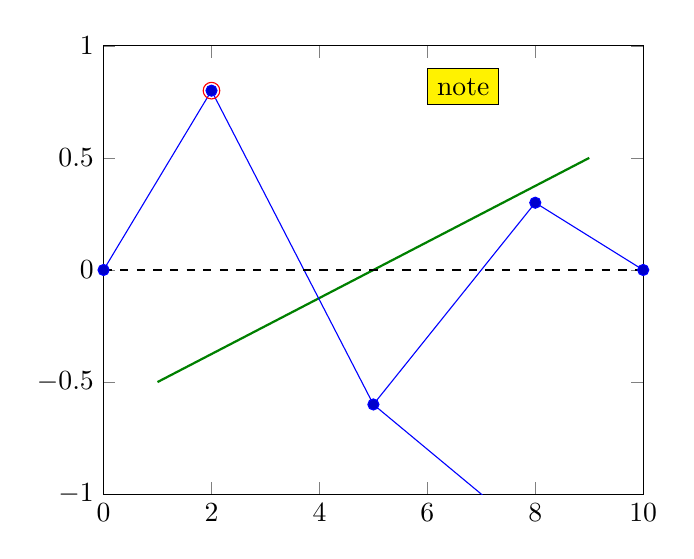
\begin{tikzpicture}
\begin{axis}[xmin=0, xmax=10, ymin=-1, ymax=1]
\draw[green!50!black, thick] (axis cs:1,-0.5) -- (axis cs:9,0.5);
\addplot coordinates {(0,0) (2,0.8) (5,-0.6) (8,0.3) (10,0)};
\draw[red] (2,0.8) circle (3pt);
\draw[dashed] (rel axis cs:0,0.5) -- (rel axis cs:1,0.5);
\node[fill=yellow, draw, anchor=north west] at (axis cs:6,0.9) {note};
\draw[blue] (5,-0.6) -- (12,-2);
\end{axis}
\end{tikzpicture}
